% Beamer slide template prepared by Tom Clark <tom.clark@op.ac.nz>
% Otago Polytechnic
% Dec 2012

\documentclass[10pt]{beamer}
\usetheme{CambridgeUS}
\usepackage{graphicx}
\usepackage{fancyvrb}


\title{Introduction to Cryptography}

\author[IN618]{Introduction to IT Security}
\institute[Otago Polytechnic]{
  Otago Polytechnic \\
  Dunedin, New Zealand \\
}
\date{}
\begin{document}

%----------- titlepage ----------------------------------------------%
\begin{frame}[plain]
  \titlepage
\end{frame}

%----------- slide --------------------------------------------------%
\begin{frame}
  \frametitle{Cryptography}

  \textbf{Cryptography} is the practice of techniques for secure communication 
  in the presence of third parties.  In particular it is about the use of
  algorithms or protocols used for secure communication.

\end{frame}


%----------- slide --------------------------------------------------%
\begin{frame}
  \frametitle{Typical uses of cryptography}

 \begin{itemize}
  \item Secure communication (including storage)
  \item Authentication 
  \item Non-repudiation
  \end{itemize}
\end{frame}



%----------- slide --------------------------------------------------%
\begin{frame}
  \frametitle{The classic process}

  \begin{figure}
    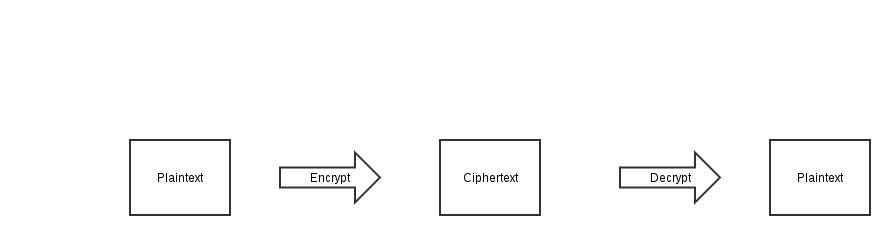
\includegraphics[scale=0.40]{encrypt-decrypt.png}
    \caption{To perform the encryption/decryption processes, \emph{keys} are required.}
  \end{figure}

\end{frame}


%----------- slide --------------------------------------------------%
\begin{frame}
  \frametitle{Some key words}

 \begin{description}
  \item[Algorithm:] the method by which we encrypt and decrypt a message
  \item [Key:] a secret used to carry out the algorithm 
  \end{description}

In order to use encryption, we need to know the algorithm and the key.
\end{frame}



%----------- slide --------------------------------------------------%
\begin{frame}
  \frametitle{Example: Caesar cipher}

 \begin{itemize}
  \item Take the letters A through Z, ignoring lower case.
  \item Shift the letters $n$ places to the right, wrapping at the end of
        the alphabet.
  \item e.g., if $n = 3$, A $\rightarrow$ D, B $\rightarrow$ E, ...
        Y $\rightarrow$ B, Z $\rightarrow$ C.
  \item In this example, the shifting is the algorithm, and the value
        of $n$ is the key.
  \end{itemize}
\end{frame}


%----------- slide --------------------------------------------------%
\begin{frame}
  \frametitle{Kerckhoffs's principle}

 \begin{itemize}
      \item A cryptographic system should be secure if everything about the system, except the key, is public knowledge.

      \item This principle is widely accepted by cryptologists.  Why?

      \item How secure is the Caesar cipher, according to this principle?

  \end{itemize}
\end{frame}



%----------- slide --------------------------------------------------%
\begin{frame}
  \frametitle{Bitwise encryption}

   Classical encryption is concerned with converting between plaintext
   and ciphertext, but modern encryption systems generally operate on 
   data as bits.
\end{frame}

%----------- slide --------------------------------------------------%
\begin{frame}[fragile]
  \frametitle{Example: XOR}

  \begin{verbatim}
      plaintext:  110010110    ciphertext:  010110001
      key:        100100111    key:         100100111
                  ---------                 ---------
      ciphertext  010110001    plaintext:   110010110
  \end{verbatim}

How secure does this seem?
\end{frame}



%----------- slide --------------------------------------------------%
\begin{frame}
  \frametitle{Symmetric encryption}

 \begin{itemize}
  \item In symmetric encryption algorithms, the same key is used
        for encryption and decryption.
  \item Symmetric algorithms are generally computationally efficient 
        and they can be very secure.
  \item The main problem with symmetric algorithms is key management.
  \end{itemize}
\end{frame}

%----------- slide --------------------------------------------------%
\begin{frame}
  \frametitle{Asymmetric encryption}

 \begin{itemize}
  \item In asymmetric encryption algorithms, different keys are used
        for encryption and decryption.
  \item Asymmetric algorithms are generally more computationally expensive
        than symmetric ones.
  \item Key management is simpler:
        \begin{itemize}
          \item To send me a message securely, encrypt it with my \emph{public                 key}, which I share freely.  Only my \emph{private key} can
                decrypt the message, but only I hold that key.
          \item If I encrypt a message with my private key, then you can
                decrypt it with my public key - and so can anybody else.
                However, since only I have the private key, I \textbf{must}
                have sent the message.
        \end{itemize}
  \end{itemize}
\end{frame}



%----------- slide --------------------------------------------------%
\begin{frame}
  \frametitle{Questions?}

  Today's lab:  Using PGP.
\end{frame}

\end{document}
